\documentclass[]{book}
\usepackage{lmodern}
\usepackage{amssymb,amsmath}
\usepackage{ifxetex,ifluatex}
\usepackage{fixltx2e} % provides \textsubscript
\ifnum 0\ifxetex 1\fi\ifluatex 1\fi=0 % if pdftex
  \usepackage[T1]{fontenc}
  \usepackage[utf8]{inputenc}
\else % if luatex or xelatex
  \ifxetex
    \usepackage{mathspec}
  \else
    \usepackage{fontspec}
  \fi
  \defaultfontfeatures{Ligatures=TeX,Scale=MatchLowercase}
\fi
% use upquote if available, for straight quotes in verbatim environments
\IfFileExists{upquote.sty}{\usepackage{upquote}}{}
% use microtype if available
\IfFileExists{microtype.sty}{%
\usepackage{microtype}
\UseMicrotypeSet[protrusion]{basicmath} % disable protrusion for tt fonts
}{}
\usepackage[margin=1in]{geometry}
\usepackage{hyperref}
\hypersetup{unicode=true,
            pdftitle={Open tools for writing open interactive textbooks (and more)},
            pdfauthor={Matthew Crump},
            pdfborder={0 0 0},
            breaklinks=true}
\urlstyle{same}  % don't use monospace font for urls
\usepackage{natbib}
\bibliographystyle{apalike}
\usepackage{color}
\usepackage{fancyvrb}
\newcommand{\VerbBar}{|}
\newcommand{\VERB}{\Verb[commandchars=\\\{\}]}
\DefineVerbatimEnvironment{Highlighting}{Verbatim}{commandchars=\\\{\}}
% Add ',fontsize=\small' for more characters per line
\usepackage{framed}
\definecolor{shadecolor}{RGB}{248,248,248}
\newenvironment{Shaded}{\begin{snugshade}}{\end{snugshade}}
\newcommand{\KeywordTok}[1]{\textcolor[rgb]{0.13,0.29,0.53}{\textbf{{#1}}}}
\newcommand{\DataTypeTok}[1]{\textcolor[rgb]{0.13,0.29,0.53}{{#1}}}
\newcommand{\DecValTok}[1]{\textcolor[rgb]{0.00,0.00,0.81}{{#1}}}
\newcommand{\BaseNTok}[1]{\textcolor[rgb]{0.00,0.00,0.81}{{#1}}}
\newcommand{\FloatTok}[1]{\textcolor[rgb]{0.00,0.00,0.81}{{#1}}}
\newcommand{\ConstantTok}[1]{\textcolor[rgb]{0.00,0.00,0.00}{{#1}}}
\newcommand{\CharTok}[1]{\textcolor[rgb]{0.31,0.60,0.02}{{#1}}}
\newcommand{\SpecialCharTok}[1]{\textcolor[rgb]{0.00,0.00,0.00}{{#1}}}
\newcommand{\StringTok}[1]{\textcolor[rgb]{0.31,0.60,0.02}{{#1}}}
\newcommand{\VerbatimStringTok}[1]{\textcolor[rgb]{0.31,0.60,0.02}{{#1}}}
\newcommand{\SpecialStringTok}[1]{\textcolor[rgb]{0.31,0.60,0.02}{{#1}}}
\newcommand{\ImportTok}[1]{{#1}}
\newcommand{\CommentTok}[1]{\textcolor[rgb]{0.56,0.35,0.01}{\textit{{#1}}}}
\newcommand{\DocumentationTok}[1]{\textcolor[rgb]{0.56,0.35,0.01}{\textbf{\textit{{#1}}}}}
\newcommand{\AnnotationTok}[1]{\textcolor[rgb]{0.56,0.35,0.01}{\textbf{\textit{{#1}}}}}
\newcommand{\CommentVarTok}[1]{\textcolor[rgb]{0.56,0.35,0.01}{\textbf{\textit{{#1}}}}}
\newcommand{\OtherTok}[1]{\textcolor[rgb]{0.56,0.35,0.01}{{#1}}}
\newcommand{\FunctionTok}[1]{\textcolor[rgb]{0.00,0.00,0.00}{{#1}}}
\newcommand{\VariableTok}[1]{\textcolor[rgb]{0.00,0.00,0.00}{{#1}}}
\newcommand{\ControlFlowTok}[1]{\textcolor[rgb]{0.13,0.29,0.53}{\textbf{{#1}}}}
\newcommand{\OperatorTok}[1]{\textcolor[rgb]{0.81,0.36,0.00}{\textbf{{#1}}}}
\newcommand{\BuiltInTok}[1]{{#1}}
\newcommand{\ExtensionTok}[1]{{#1}}
\newcommand{\PreprocessorTok}[1]{\textcolor[rgb]{0.56,0.35,0.01}{\textit{{#1}}}}
\newcommand{\AttributeTok}[1]{\textcolor[rgb]{0.77,0.63,0.00}{{#1}}}
\newcommand{\RegionMarkerTok}[1]{{#1}}
\newcommand{\InformationTok}[1]{\textcolor[rgb]{0.56,0.35,0.01}{\textbf{\textit{{#1}}}}}
\newcommand{\WarningTok}[1]{\textcolor[rgb]{0.56,0.35,0.01}{\textbf{\textit{{#1}}}}}
\newcommand{\AlertTok}[1]{\textcolor[rgb]{0.94,0.16,0.16}{{#1}}}
\newcommand{\ErrorTok}[1]{\textcolor[rgb]{0.64,0.00,0.00}{\textbf{{#1}}}}
\newcommand{\NormalTok}[1]{{#1}}
\usepackage{longtable,booktabs}
\usepackage{graphicx,grffile}
\makeatletter
\def\maxwidth{\ifdim\Gin@nat@width>\linewidth\linewidth\else\Gin@nat@width\fi}
\def\maxheight{\ifdim\Gin@nat@height>\textheight\textheight\else\Gin@nat@height\fi}
\makeatother
% Scale images if necessary, so that they will not overflow the page
% margins by default, and it is still possible to overwrite the defaults
% using explicit options in \includegraphics[width, height, ...]{}
\setkeys{Gin}{width=\maxwidth,height=\maxheight,keepaspectratio}
\IfFileExists{parskip.sty}{%
\usepackage{parskip}
}{% else
\setlength{\parindent}{0pt}
\setlength{\parskip}{6pt plus 2pt minus 1pt}
}
\setlength{\emergencystretch}{3em}  % prevent overfull lines
\providecommand{\tightlist}{%
  \setlength{\itemsep}{0pt}\setlength{\parskip}{0pt}}
\setcounter{secnumdepth}{5}
% Redefines (sub)paragraphs to behave more like sections
\ifx\paragraph\undefined\else
\let\oldparagraph\paragraph
\renewcommand{\paragraph}[1]{\oldparagraph{#1}\mbox{}}
\fi
\ifx\subparagraph\undefined\else
\let\oldsubparagraph\subparagraph
\renewcommand{\subparagraph}[1]{\oldsubparagraph{#1}\mbox{}}
\fi

%%% Use protect on footnotes to avoid problems with footnotes in titles
\let\rmarkdownfootnote\footnote%
\def\footnote{\protect\rmarkdownfootnote}

%%% Change title format to be more compact
\usepackage{titling}

% Create subtitle command for use in maketitle
\newcommand{\subtitle}[1]{
  \posttitle{
    \begin{center}\large#1\end{center}
    }
}

\setlength{\droptitle}{-2em}
  \title{Open tools for writing open interactive textbooks (and more)}
  \pretitle{\vspace{\droptitle}\centering\huge}
  \posttitle{\par}
  \author{Matthew Crump}
  \preauthor{\centering\large\emph}
  \postauthor{\par}
  \predate{\centering\large\emph}
  \postdate{\par}
  \date{2018-03-09}

\usepackage{booktabs}
\usepackage{amsthm}
\makeatletter
\def\thm@space@setup{%
  \thm@preskip=8pt plus 2pt minus 4pt
  \thm@postskip=\thm@preskip
}
\makeatother

\usepackage{amsthm}
\newtheorem{theorem}{Theorem}[chapter]
\newtheorem{lemma}{Lemma}[chapter]
\theoremstyle{definition}
\newtheorem{definition}{Definition}[chapter]
\newtheorem{corollary}{Corollary}[chapter]
\newtheorem{proposition}{Proposition}[chapter]
\theoremstyle{definition}
\newtheorem{example}{Example}[chapter]
\theoremstyle{definition}
\newtheorem{exercise}{Exercise}[chapter]
\theoremstyle{remark}
\newtheorem*{remark}{Remark}
\newtheorem*{solution}{Solution}
\begin{document}
\maketitle

{
\setcounter{tocdepth}{1}
\tableofcontents
}
\chapter*{Preface}\label{preface}
\addcontentsline{toc}{chapter}{Preface}

This is a tutorial and set of working examples for creating web-based
textbooks using a collection of open-source tools.

This web-book is itself a working example. All of the source code needed
to compile this book yourself is included in the
\href{https://github.com/CrumpLab/OER_bookdown}{github repository for
this book}. So, you could download the repository, and by following the
instructions laid out across the chapters, replace this text with your
own, and then compile your book as a web-page, .pdf or epub.

\chapter{Overview}\label{overview}

\section{Open online educational resources
(OERs)}\label{open-online-educational-resources-oers}

OERs are educational resources that are public and freely available to
students (or anyone) through the web. There are already numerous OER
databases linking to numerous free textbooks across many domains of
study (e.g., \href{http://libguides.brooklyn.cuny.edu/research/oer}{see
the BC library OER site}). These texts are often disseminated under a
creative commons license, which allows anyone to mix, match, edit,
update, and transform those texts, and then share them again with the
public at large under the same license. Finding existing OERs can be a
good starting point for developing your own content.

\section{What is this tutorial?}\label{what-is-this-tutorial}

This tutorial shows how a few open-source tools can be brought together
for quicky developing and sharing content in the form of online books
and webpages. The tools require some downloading of free programs (all
cross-platform), but once in place, allow you to write and format text
with minimal syntax, and then easily compile your source documents into
multiple formats, including web-books, .pdf's, and e-pubs.

\begin{figure}[htbp]
\centering
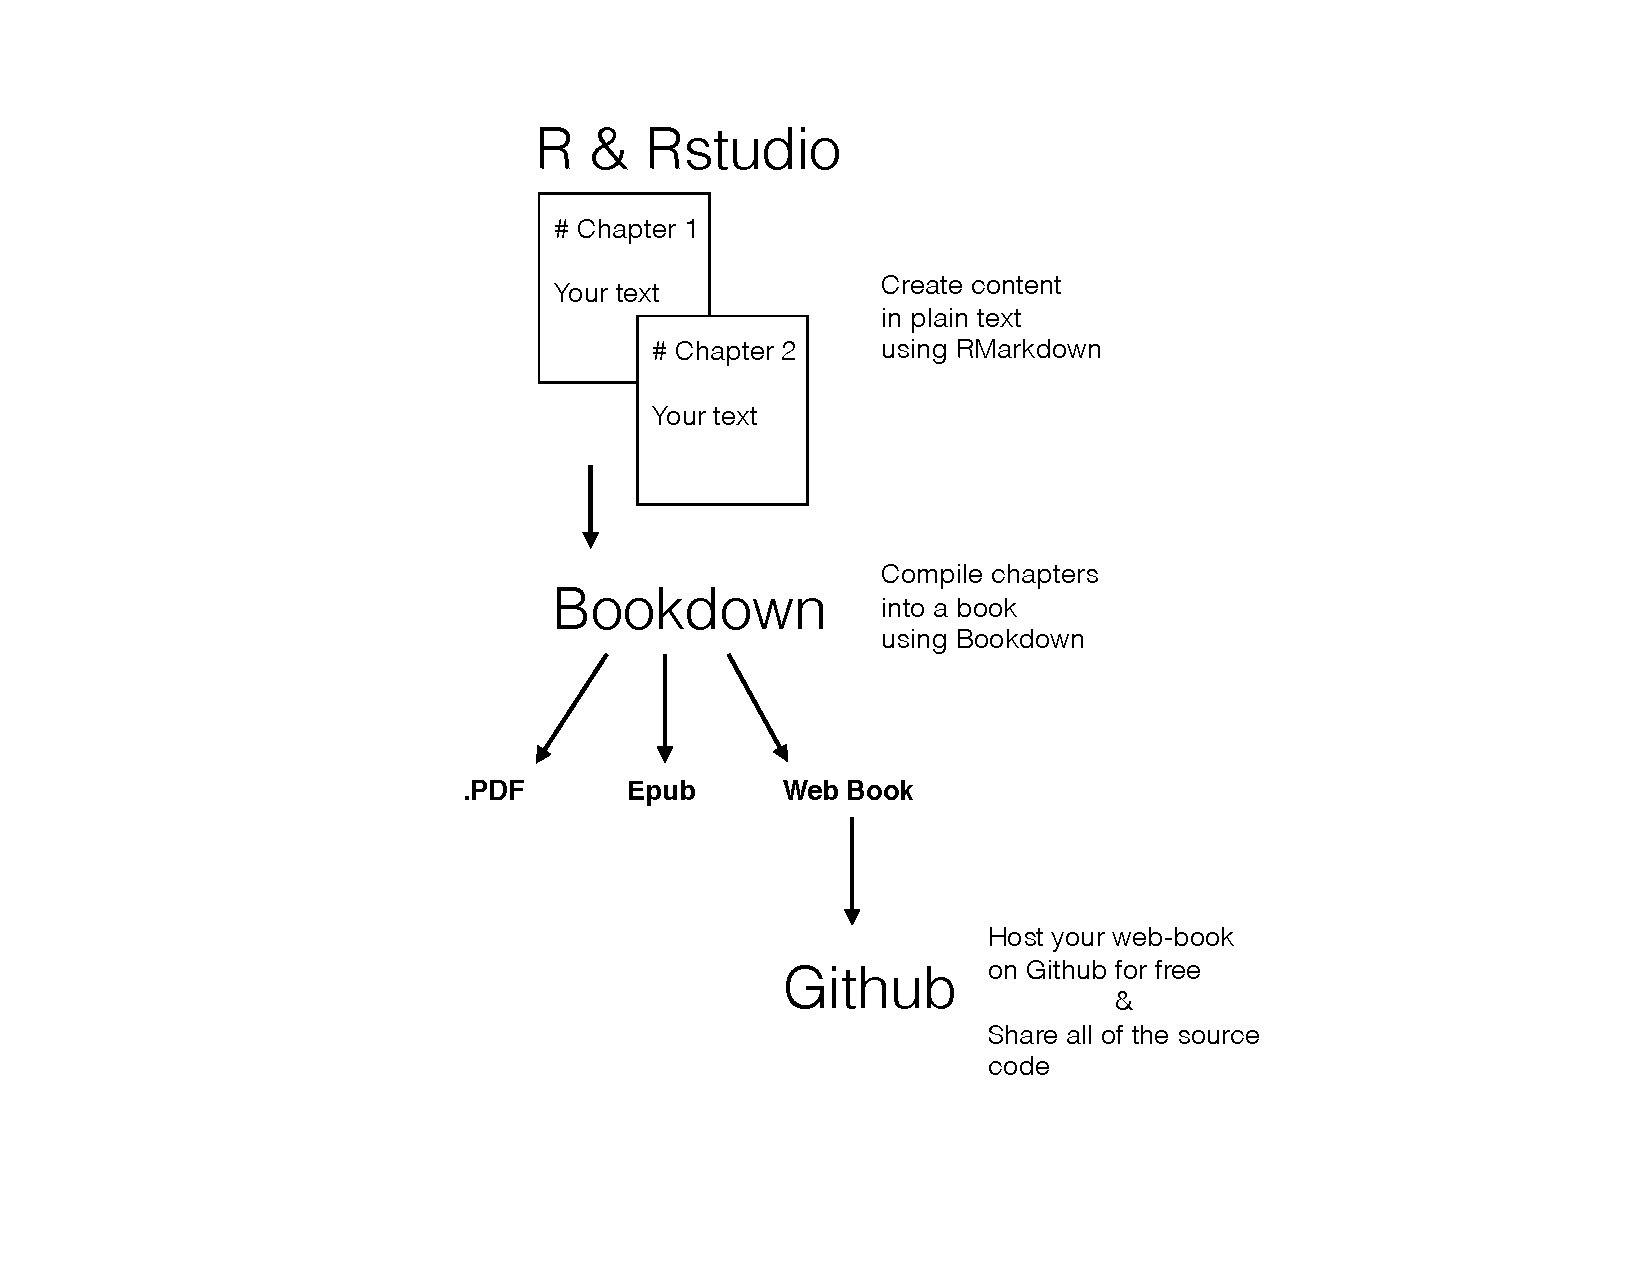
\includegraphics{Figures/OERTutorial_Overview.pdf}
\caption{\label{fig:fig1}Basic steps}
\end{figure}

This tutorial also covers tools to enhance student interaction with the
content, including the ability for students to select text in a web-book
and then post comments about the text. Depending on the pedagogical
goals of the instructor, posts could be to critically evaluate portions
of the textbook, supplement sections with additional examples, and tag
sections in need of revision or that were particularly helpful. All of
these comments can be made publically accessible so that everyone
viewing the textbook can see all of the comments as they are posted
(inline, corresponding to the sections that were annotated).
Furthermore, the database of annotations can easily be extracted and
used for revising the text, or other purposes.

\section{Can I see an example of what you are talking
about?}\label{can-i-see-an-example-of-what-you-are-talking-about}

Yes, there are many working examples already. As the preface mentions,
this tutorial is an example. So the bells and whistles you see here
constitute one example of an end product. Some additional examples
include a \href{https://crumplab.github.io/ResearchMethods/}{Research
Methods for Psychologist's textbook}, and a
\href{https://crumplab.github.io/programmingforpsych/}{Programming for
Psychology textbook} that I made using the tools in this tutorial.

If you want to see examples of the inline commenting features, simply
follow the directions in the preface of the above two books. Inline
commenting is made possible by the
\href{https://web.hypothes.is}{hypothes.is} browser add-on tool. It is
simple to install, requiring that you sign up with hypothesis, and then
follow their directions to install an add-on for chrome, or a
bookmarklet for other browsers. When you turn on hypothesis viewing
these web-books, you will be able to see any public comments made by
other people.

\section{The toolbox (what do I need to
download)}\label{the-toolbox-what-do-i-need-to-download}

Each of the chapters in this tutorial will discuss each of these tools
in more depth, along with links to many helpful tool-specific resources
already available online.

\subsection{R}\label{r}

\href{https://www.r-project.org}{R} is a free and open-source
programming language primarily developed for statistical analysis. R has
a large community of active open-source developers who are makin R
better and more powerful everyday. R comes with existing packages for
statistical analysis, but can be extended to accomplish many more tasks
by downloading and installing additional packages. Download and install
before you download and install R-studio.

\subsection{R-studio}\label{r-studio}

\href{https://www.rstudio.com}{R-Studio} is a free and open-source GUI
for R. For those of you familiar with the Matlab environment, R-studio
looks similar.

\subsection{Markdown and R Markdown}\label{markdown-and-r-markdown}

\href{https://github.com/adam-p/markdown-here/wiki/Markdown-Cheatsheet}{Markdown}
is a simple mark-up language for creating .html files viewable in
web-browsers. HTML (hyper-text markup language) is a powerful, but
visually cluttered syntax for creating content to be displayed in
web-pages. Markdown allows you to easily write text while avoiding
writing html syntax. For example, This document is written in markdown.

\href{http://rmarkdown.rstudio.com}{RMarkdown} is R's version of
markdown. It's basically the same as markdown, but allows you to inject
and run R code inside a markdown document. This is especially useful
when you are writing documents that contain output from data-analysis
you have conducted in R. This document is an .Rmd file (Rmarkdown). The
paragraphs are plain text, and the header's (level I, II, III) are
defined by \#'s.

\subsection{Bookdown}\label{bookdown}

\href{https://bookdown.org/yihui/bookdown/}{Bookdown} is an R package
for compiling Rmarkdown documents into various formats, including
web-books, .pdf's, and epubs. This incredible package, along with the
knitr package, does much of the heavy lifting, allowing writer's to
focus on content generation, rather than the technical details of
deploying that content to the various formats. Once the .Rmd files are
written, deployment can is a single-click. Bookdown also provides
different formats for styling the output, and styling is customizable.

\subsection{Github}\label{github}

\href{https://github.com}{Github} is a version control software
development tool/website. Github provides a free option for hosting
static web-pages (e.g., you could deploy your web-book to github), and
allows you to store the source code for generating your book in an
online repository. This allows others to easily copy your source code
and make suggested edits that you can incorporate back into your
content. This web-book is hosted using github pages, and the source code
for this book is hosted in a github repository. Downloading the github
repository will give you all the files you need to compile this book,
and by editing the text in this book, you can change it into your own.

\subsection{Hypothes.is}\label{hypothes.is}

\href{https://web.hypothes.is}{Hypothes.is} is a web-browser add-on for
annotating the web via inline commenting. This allows anyone to select a
snippet of text in a web-browser and then post a comment about the
selected text. Annotations can be made publicly or privately. All public
annotations can be viewed by anyone else running hypothesis on the same
website. Using Hypothesis with your web-book allows you to engage
students in interacting with the textbook by allowing them to contribute
to content generation (by posting new content), or content revision (by
tagging sections in need of revision).

\subsection{hypothesisr}\label{hypothesisr}

\href{https://github.com/mdlincoln/hypothesisr}{hypothesisr} is an r
package for scraping annotation data collected through the hypothesis
app. This could be used for identifying tagged sections in need of
revision, or for other analytic purposes.

\subsection{Zotero}\label{zotero}

\href{https://www.zotero.org}{Zotero} is a free and open source citation
management tool. It is cloud-based with both browser and app versions.
It is easy to create .pdf libraries along with citation information, and
then compile bibliographies with citation keys for quickly citing
articles. The R bookdown package is compatible with latex-style
bibliography files that can be exported by Zotero.

\section{Quickstart}\label{quickstart}

If you want to skip to getting up and running, follow these steps. If
they all work, then you should be able to copy the source code this
book, compile it and display it as a webbook (or pdf or epub), and then
start modifying the text content to create your own resources.

\subsection{Download all the programs, and set-up needed
accounts}\label{download-all-the-programs-and-set-up-needed-accounts}

\begin{enumerate}
\def\labelenumi{\arabic{enumi}.}
\tightlist
\item
  Download and install R
\item
  Download and install R-studio
\item
  Open R-studio, choose the packages tab, search for the package
  ``bookdown'', download and install
\item
  Create an account with Github
\item
  Download and install Github Desktop
\end{enumerate}

\subsection{Create a Github
repository}\label{create-a-github-repository}

\begin{enumerate}
\def\labelenumi{\arabic{enumi}.}
\setcounter{enumi}{5}
\tightlist
\item
  Create a new repository on the Github website, give it a name
\item
  Clone the repository to your local computer using Github Desktop
\item
  Open the local repository
\end{enumerate}

\subsection{Copy and compile this
repository}\label{copy-and-compile-this-repository}

\begin{enumerate}
\def\labelenumi{\arabic{enumi}.}
\setcounter{enumi}{8}
\tightlist
\item
  Download this repository as a .zip file to your computer
\item
  Copy the contents of the folder to your new local folder for your
  github repository
\item
  In Github Desktop you should now see that there are many new changes
  to your repository. Commit the changes (uploads them to the online
  repository)
\item
  Open the OERbookdown.Rproj in Rstudio, this is an R project file that
  will automatically point R to the files in this folder.
\item
  In Rstudio, on the top right panel, choose the Build tab, then click
  build book.
\item
  If everything goes smoothly, you will have compiled this book
\end{enumerate}

\chapter{R, R-studio, and RMarkdown}\label{r-r-studio-and-rmarkdown}

\section{Quick start steps}\label{quick-start-steps}

\begin{enumerate}
\def\labelenumi{\arabic{enumi}.}
\tightlist
\item
  Download and install \href{https://www.r-project.org}{R} for your
  platform
\item
  Download and install \href{https://www.rstudio.com}{R-Studio} for your
  platform (R must be installed first)
\item
  Open R-studio
\item
  Open a new RMarkdown document, compile it using the knit button.
\end{enumerate}

\section{R Markdown}\label{r-markdown}

You can open a new R Markdown (.rmd) file from Rstudio through the file
menu (New File -\textgreater{} R markdown\ldots{}), or by clicking the
green plus sign icon in the top left-hand corner of R-studio, and
choosing R Markdown. This will open a window allowing you to name your
new document, and then will open the new R Markdown document in the
R-studio text editor. The new document shows some example syntax for
writing in R Markdown. You can compile the document to see what it will
look like as a .pdf or website by clicking the \textbf{Knit} button.

R Markdown offers a convenient way to create content in plain-text, and
then display the content as a .pdf or web-page. R Markdown separates
content from style. In a typical word-processor, like Microsoft Word, an
author formats the style of the content as they create it, the two are
bound together. In an R Markdown document the content is written in
plain text without any styling. In a second step, the R Markdown
document is compiled to display the content in a particular style. This
tutorial uses the styles available in the
\href{https://bookdown.org/yihui/bookdown/}{bookdown} package. There are
other styles available, and you can create and modify your own styles.

R Markdown is commonly used to create notebooks for the results of
statistical analysis in R. R Markdown allows an author to write sections
of text, together with sections of R code. When the document is
compiled, it is displayed as a formatted document with sections of
headers and text, interspersed with sections of the R code used to run
analyses, along with the output of the analyses. For example, below is a
snippet of R code that computes and then displays the mean for the set
of numbers 1 to 10.

\begin{Shaded}
\begin{Highlighting}[]
\KeywordTok{mean}\NormalTok{(}\KeywordTok{seq}\NormalTok{(}\DecValTok{1}\NormalTok{,}\DecValTok{10}\NormalTok{,}\DecValTok{1}\NormalTok{))}
\end{Highlighting}
\end{Shaded}

\begin{verbatim}
## [1] 5.5
\end{verbatim}

Although reporting statistical analyses may be the most common use of R
Markdown, the framework can also be used to build books, using the
\href{https://bookdown.org/yihui/bookdown/}{bookdown} package.

\section{R Markdown tips}\label{r-markdown-tips}

I recommend looking at examples of .rmd files to see how they work. For
example, all of the chapters in this tutorial are written in R Markdown
using .rmd files. So, you can view the source code for each chapter by
opening the .rmd file corresponding to each chapter. You will find the
syntax to be fairly basic. Chapter headings are lines preceded by a \#.
Section headers, and sub, or sub-sub headers, are lines preceded by
\#\#, \#\#\#, or \#\#\#\#. Paragraphs are new lines with text. You will
also see how to insert hyperlinks to websites, as well as insert
graphics.

\subsection{Inserting Graphics}\label{inserting-graphics}

In the repository for this book, you will find a Figures file. You can
place .png and .pdf files in this folder. Then, to insert a graphic you
create a short R code snippet, and point R toward the location of the
file. See the Figure 1 example in the Overview.Rmd file.

\subsection{Inserting References}\label{inserting-references}

See the chapter on Zotero.

\subsection{Links for using R
Markdown}\label{links-for-using-r-markdown}

\begin{enumerate}
\def\labelenumi{\arabic{enumi}.}
\tightlist
\item
  The R-studio website has in-depth tutorials on using R Markdown,
  available \href{http://rmarkdown.rstudio.com/lesson-1.html}{here}.
\item
  \href{http://rmarkdown.rstudio.com/lesson-15.html}{Cheatsheet for R
  Markdown}
\item
  In the Help menu of R-Studio, you can also find cheetsheats and
  formatting guides for using R Markdown.
\end{enumerate}

\chapter{Bookdown}\label{bookdown-1}

\href{https://bookdown.org/yihui/bookdown/}{Bookdown} is an R package
written by Yihui Xie. Bookdown is a tool for stitching together multiple
R Markdown files into a whole book. Most impressive, is that the final
product can rendered in multiple formats, including .pdf, epub, and as a
web-page.

\section{R Packages and installing
Bookdown}\label{r-packages-and-installing-bookdown}

R is an open-source platform. Many developers create and share packages
for accomplishing different tasks in R.

Packages can be installed in R-Studio by clicking the packages tab in
the lower right-hand window, and then clicking the Install button. If
you know the name of the package you want to install, then type it in,
and click install.

To install bookdown, type bookdown into the textbox, make sure you have
``install dependencies'' clicked on, and then press install.

The \textbf{packages} tab also shows all of the currently installed R
packages on your system. These packages needed to be loaded, or turned
on, in order to use them. You can do this by clicking on the checkmark
box beside each package.

You may into a situation where your R Markdown file does not compile,
and you get a message saying that a particular package is required.
Usually this can be resolved by installing the missing package, using
the same method used to install the bookdown package.

\section{Using Bookdown}\label{using-bookdown}

Yihui Xie has written a whole
\href{https://bookdown.org/yihui/bookdown/}{tutorial book}, using
bookdown, to describe how to use the bookdown package. Similarly, check
out Yihui Xie's
\href{https://bookdown.org/yihui/bookdown/get-started.html}{minimal
working example}, which contains all of the source code necessary to
compile a barebones book.

Similarly, this tutorial was written in bookdown, and is intended to be
used as a starting point for you to create your own book.

\section{Compiling this tutorial using
bookdown.}\label{compiling-this-tutorial-using-bookdown.}

\begin{enumerate}
\def\labelenumi{\arabic{enumi}.}
\tightlist
\item
  Download the Github Repository for this tutorial as a .zip file here.
\item
  Unzip the file somewhere on your computer.
\item
  Open R-Studio
\item
  Navigate to the tutorial folder using the Files tab
\item
  Open the R Markdown file \textbf{index.Rmd} and click the button
  \textbf{Build Book} on the \textbf{Build} tab of RStudio (top
  right-hand corner).
\end{enumerate}

You can build the book as a .pdf, epub, or gitbook (renders as a
web-page in the gitbook style). After you build the book, it should
pop-up in a viewer screen.

\chapter{Github}\label{github-1}

To quote from wikipedia, ``Github is a Web-based Git version control
repository hosting service. It is mostly used for computer code.''---
and I would add, many other things.

The purpose of this chapter is to describe how Github can be used to
serve your web-book (compiled using bookdown), and to share the source
code so that others can duplicate and modify your book, or so that
others can contribute content to your existing book.

\section{Getting Started}\label{getting-started}

\subsection{Make an account with
Github}\label{make-an-account-with-github}

To get started with \href{https://github.com}{Github} you need to create
a free account. You should see a sign up option on the main page.

Your account now consists of your profile page (where you can add
information about yourself), and an empty list of repositories.
Repositories are Github file folders. They can be purely cloud-based;
for example, you can create a repository then add files to it through
the web-based interface. You can also create a copy of each repository
on your local computer, make changes to the repository on your local
computer, and then merge those changes with the online repository.

\subsection{Install Github Desktop}\label{install-github-desktop}

Github has provided a free and convenient tool for using your local
computer to interface with the web-based version of Github. To use the
tool, download and install the \href{https://desktop.github.com}{desktop
app for Github}. Once the app is installed, make sure that you
\href{https://help.github.com/desktop/guides/getting-started-with-github-desktop/authenticating-to-github/}{connect
it to your Github account} so that you can access repositories that you
create.

\chapter{Repository workflow}\label{repository-workflow}

We will use the following workflow:

\begin{enumerate}
\def\labelenumi{\arabic{enumi}.}
\tightlist
\item
  Create a new empty repository on the Github Website
\item
  Clone the repository to your local computer
\item
  Add files to the repo on your local computer (work locally)
\item
  Merge the files back to the Github Website (share final versions)
\end{enumerate}

\section{Creating a new repository on
Github.com}\label{creating-a-new-repository-on-github.com}

\begin{enumerate}
\def\labelenumi{\arabic{enumi}.}
\tightlist
\item
  Log in to Github.com
\item
  In the top right corner of the page, click the ``+'' icon
\item
  Choose new repository
\item
  Give it a short name
\item
  You have a few other options that you can revisit later
\item
  Click create repository
\end{enumerate}

\section{Cloning a copy on your
computer}\label{cloning-a-copy-on-your-computer}

\begin{enumerate}
\def\labelenumi{\arabic{enumi}.}
\tightlist
\item
  Open the Github desktop app
\item
  Login in to your Github account
\item
  Choose the clone repository option
\item
  Find the name of the repository you created on Github and select it.
  Github Desktop will now download the contents of the repository and
  save it locally (in the file folder of your choice) on your computer
\end{enumerate}

\section{Make changes to the
repository}\label{make-changes-to-the-repository}

\begin{enumerate}
\def\labelenumi{\arabic{enumi}.}
\tightlist
\item
  If you are on a mac, choose ``show in finder''.
\item
  You can now edit any of the files locally
\end{enumerate}

\section{Update the online github
repository}\label{update-the-online-github-repository}

\begin{enumerate}
\def\labelenumi{\arabic{enumi}.}
\tightlist
\item
  Any time you change a file, git will track all of the changes that you
  make
\item
  To submit changes, choose the commit button
\item
  All of your changes will now be uploaded to the online repository.
\end{enumerate}

\chapter{Hypothes.is}\label{hypothes.is-1}

\href{https://web.hypothes.is}{Hypothes.is} is a web-browser add-on for
annotating the web via inline commenting. This allows anyone to select a
snippet of text in a web-browser and then post a comment about the
selected text. Annotations can be made publicly or privately. All public
annotations can be viewed by anyone else running hypothesis on the same
website. Using Hypothesis with your web-book allows you to engage
students in interacting with the textbook by allowing them to contribute
to content generation (by posting new content), or content revision (by
tagging sections in need of revision).

If you publish your bookdown book as a webpage, then you anyone with
Hypothes.is can use it to annotate the textbook.

\section{A case study example}\label{a-case-study-example}

I recently compiled a
\href{http://crumplab.github.io/ResearchMethods/}{Research Methods in
Psychology textbook} using the tools described in this tutorial. The
landing page describes how Hypothes.is can be used in conjunction with
the textbook.

In class I assigned students the task of downloading Hypothes.is,
creating a Hypothes.is account, and then throughout the course gave them
various assignments where they were responsible for annotating parts of
the textbook.

For example, in one assignment I had students annotate sections of the
textbook that were in need of improvement. This allows students to
participate in content revision as they read the textbook. Other
assignments could include focused online discussion about textbook
content using annotations, or using annotations as a way for students to
add content to the textbook.

\section{hypothesisr}\label{hypothesisr-1}

\href{https://github.com/mdlincoln/hypothesisr}{hypothesisr} is an r
package for scraping annotation data collected through the hypothesis
app. All public annotations submitted through hypothesis to any website
are publically available for download. As a result, the hypothesisr
package can be used to download and process the annotations submitted to
your website.

As a part of this project, we have created a Shiny app that conveniently
displays and manipulates hypothesis annotation databases in a website.
The Shiny app is located in this github repository.

\chapter{Zotero}\label{zotero-1}

\href{https://www.zotero.org}{Zotero} is a free, cross-platform tool to
help you collect, organize, cite, and share your research sources.
Zotero is similar to Mendeley or EndNote.

The purpose of this chapter is to show how Zotero can be used as a
reference manager to allow you to cite works in your book, and
automatically compile bibliographies or reference sections. The bookdown
package uses Latex bibliography files to generate citations and create
bibliographies. These .bib files are text-based files with a specific
syntax for coding the relevant information in a citation. Each citation
in a .bib file has an associated key that is inserted into an Rmarkdown
document to generate a citation. We will use Zotero to avoid writing our
own .bib from scratch. Instead, there are convenient methods for
populating Zotero with a database of references, and for compiling a
.bib file from a Zotero databse that can be used in bookdown.

\section{Getting Started}\label{getting-started-1}

\begin{enumerate}
\def\labelenumi{\arabic{enumi}.}
\tightlist
\item
  Create an account with \href{https://www.zotero.org}{Zotero}, click
  register in the top-right corner
\item
  \href{https://www.zotero.org/download/}{Download} the Zotero Desktop
  app
\item
  \href{https://www.zotero.org/download/}{Download} the Zotero Connector
  extension for your web-browser
\end{enumerate}

Zotero operates on the cloud as well as on your desktop. You can connect
your online Zotero account with your desktop app in the preferences.

\section{Populating Zotero with
references}\label{populating-zotero-with-references}

There are multiple ways to import references into Zotero. In the Zotero
desktop app you can create folders to organize your references.

\subsection{Drag and Drop .pdfs}\label{drag-and-drop-.pdfs}

\begin{enumerate}
\def\labelenumi{\arabic{enumi}.}
\tightlist
\item
  Create a new folder and name it
\item
  Drag and drop .pdfs into the folder
\item
  Highlight the .pdfs, then right-click, and choose ``retrieve metadata
  for pdf''.
\item
  For most journal articles, Zotero will be able to automatically find
  the citation information for your .pdf. This will convert the .pdf
  into a Zotero citation that includes both the citation information, as
  well as the .pdf
\end{enumerate}

\subsection{Import citations and pdfs from the
web}\label{import-citations-and-pdfs-from-the-web}

\begin{enumerate}
\def\labelenumi{\arabic{enumi}.}
\tightlist
\item
  Ensure that your Desktop app is open, and that you have installed the
  Zotero plugin for your web-browser
\item
  Use google scholar to search for an article
\item
  Click the Zotero button in your web-browser
\item
  You should see a list of all of the articles on the google scholar
  page.
\item
  Click any or all the articles you want to import, then import them
\item
  Zotero will download the citation information along with any
  associated .pdf to the current folder that is open in the Zotero
  desktop app.
\end{enumerate}

Zotero is fairly flexible, so the above process will generally work when
you are accessing many different databases, and journal web-pages for
specific articles.

\subsection{A note of caution}\label{a-note-of-caution}

The citation information that Zotero downloads is sometimes inaccurate.
Be sure to check the fields for each of your citations to ensure they
are accurate. For example, page ranges are often missing.

\section{Generating a .bib file}\label{generating-a-.bib-file}

\begin{enumerate}
\def\labelenumi{\arabic{enumi}.}
\tightlist
\item
  Right-click a Zotero folder
\item
  Choose ``Export Collection''
\item
  Choose ``Bibtex''
\item
  Save the file
\item
  Copy the file into the folder for your bookdown project
\item
  add the file to the bibliography line in the Index.Rmd file.
\end{enumerate}

\section{Citing references in an RMarkdown
file}\label{citing-references-in-an-rmarkdown-file}

Citations are add using the following format \texttt{@citationkey}, or
\texttt{{[}@citationkey{]}} to place the author,year citation in
parentheses. The citation key name is listed for each citation in the
bib file. Here are a couple of links with some additional examples:
\href{https://bookdown.org/yihui/bookdown/citations.html}{examples from
bookdown}, and examples from
\href{http://rmarkdown.rstudio.com/authoring_bibliographies_and_citations.html}{RMarkdown}.

The source code for this book contains two .bib files: book.bib and
packages.bib. Each citation in those files has an associated citation
key. Here is an example of citing the bookdown package \citep{xie2015}.
This is an example of citing R-core team \citep{R-base}

\subsection{Cite while you write}\label{cite-while-you-write}

A minor inconvenience when using .bib for citations in Rmarkdown is that
you have to know the citation key, and these are easy to forget. One
option is to load up your .bib file, then search through it to find the
citation key.

Another option is to download and install the \texttt{citr} package.
Once this package is installed, you can use its cite while your write
feature. Click the tools menu, addins, then, insert citations. This will
open up a window showing all of the citations in your bib files. You can
click multiple citations, and then insert the citation keys into your
Rmarkdown document. This is convenient method for quickly finding needed
citation keys. I recommend first openining the index.rmd file (which
points to your .bib files), and then opening the insert citations tools;
this will allow the tool to find your .bib files. After this point, you
should be able to use the tool when you are working within .Rmd files
for each chapter.

\bibliography{book.bib,packages.bib}


\end{document}
